\newpage
\section{Analiza problemu}		%2
%Napisać gdzie używa się tego algorytmu
%Opisać sposób działania programu/algorytmu
%Napisać spsoób wykorzystania algorytmu po przez wykonanie przykładu (np. mnożenie macierzy - wykonać ręcznie przykład z mnożeniem macierzy pokazujący jak mnoży się macierz ręcznie)
%Jeśli zadanie zakłada przedstawienie jakiegoś narzędzia (np. git, AI) należy opisać narzędzie

\subsection{Algorytm obliczania $\pi$ metodą całkowania numerycznego}

Algorytm obliczania $\pi$ metodą całkowania numerycznego (połączenie metody Archimedesa\cite{archimedes} i sum Riemanna\cite{riemannwiki}) polega na wykorzystaniu wzoru na pole koła \[P = \pi r^2,\] Wzór ten można przekształcić do postaci \[\pi = \frac{P}{r^2},\] gdzie $P$ to pole koła, a $r$ to promień. Z tej relacji wynika, że można użyć wartości promienia i pola koła do obliczenia $\pi$. Jeżeli wiadomo jaki jest promień koła, do określenia pola pod łukiem ćwiartki okręgu i pomnożenia wyniku przez 4 (dlatego, że koło jest symetryczne względem osi $x$ i $y$ układu współrzędnych). Funkcję określająca kształt łuku ćwiartki można uzyskać poprzez przekształcenie wzoru okrąg \[x^2 + y^2 = r^2,\] gdzie $x$, $y$ to koordynaty punktów na okręgu, a $r$ to promień. Przekształcając wzór do postaci $f(x,r) \to y$ uzyskujemy \[y = \sqrt{r^2 - x^2},\] gdzie $y, x \geq 0$ (dlatego, że obliczana jest tylko ćwiartka). Pole pod tą funkcją to całka oznaczona \[P_{cw} = \int_{0}^{r} \sqrt{r^2 - x^2} \,dx.\] Pole całego koła to byłoby zatem \[P = 4P_{cw}.\]

Należy natomiast zauważyć, że nie da się obliczyć dokładnej wartości tej całki bez wykorzystania liczby $\pi$. Dlatego, należy skorzystać z sum Riemanna\cite{riemannwiki}, aby obliczyć aproksymację wartości $\pi$, poprzez podkładanie prostokątów z szerokością o danej wartości i wysokości określonej poprzez wartość funkcji $y = \sqrt{r^2 - x^2}$, gdzie $x$ to punkty oddzielone od siebie o daną szerokość.

Jeżeli jako promień przyjmie się 1, to \[\pi = \frac{P}{1^2} \implies \pi = P.\] To założenie upraszcza kalkulacje, ponieważ nie trzeba dzielić pola.

\subsection{Git}
Kolejnym konceptem, którym zajmuje się projekt jest narzędzie git\cite{gitsite}. Pozwala ono zarządzać poszczególnymi wersjami projektów. Głównym korzeniem gita jest system commitów, czyli zapisania zmian w pliku w stosunku do commita starszego. To, w połączeniu z jego innymi możliwościami pozwala na tworzenie długich i skomplikowanych osi czasu danych projektów. 

Użycie gita można zademonstrować na prostym przykładzie. Tworzymy katalog a w nim repozytorium, uzywając komendy \texttt{git init}, jak widać na rys. \ref{fig:git_init}.

\begin{figure}[H]
	\centering
	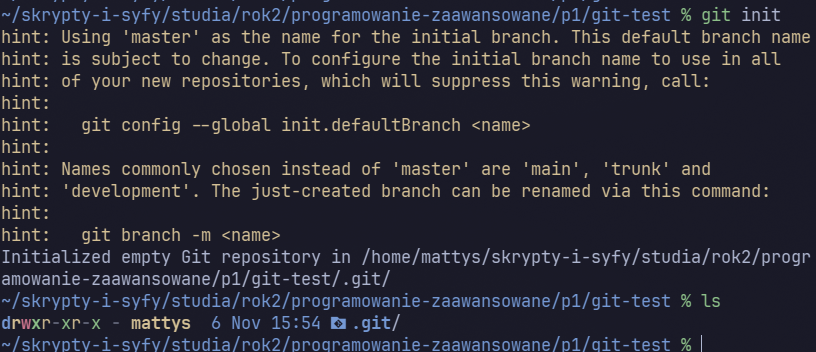
\includegraphics[width=1\textwidth]{images/git_init.png}
	\caption{\centering{Puste repozytorium git}}
	\label{fig:git_init}
\end{figure}

Stwórzmy jakiś plik i dodajmy go do repozytorium. Plik można dodać do repozytorium komendą \texttt{git add}

\begin{figure}[H]
	\centering
	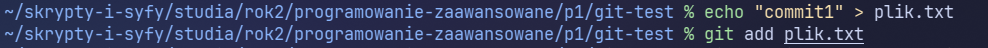
\includegraphics[width=1\textwidth]{images/git_add.png}
	\caption{\centering{Stworznie pliku w repozytorium}}
	\label{fig:git_add}
\end{figure}

Następnie należy scommitować zmiany. 

\begin{figure}[H]
	\centering
	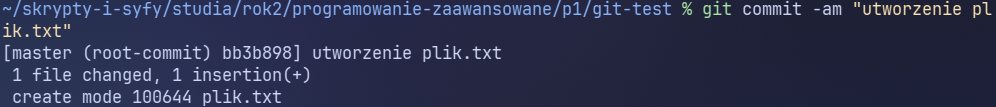
\includegraphics[width=1\textwidth]{images/git_commit1.png}
	\caption{\centering{Commit nr. 1}}
	\label{fig:git_commit1}
\end{figure}

Na rysunku \ref{fig:git_commit1} użyta komenda \texttt{git commit} commituje wszystkie dodane pliki (\texttt{-a}) z jakimś komunikatem (\texttt{-m}).  

\begin{figure}[H]
	\centering
	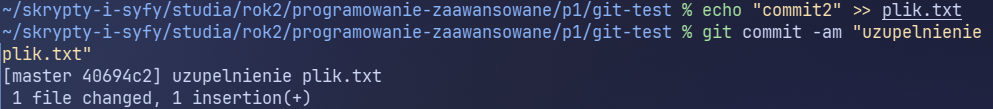
\includegraphics[width=1\textwidth]{images/git_commit2.png}
	\caption{\centering{Commit nr. 2}}
	\label{fig:git_commit2}
\end{figure}

Na rys. \ref{fig:git_commit2}, został utworzony kolejny commit, dodajacy zmiany do \texttt{plik.txt}.

\begin{figure}[H]
	\centering
	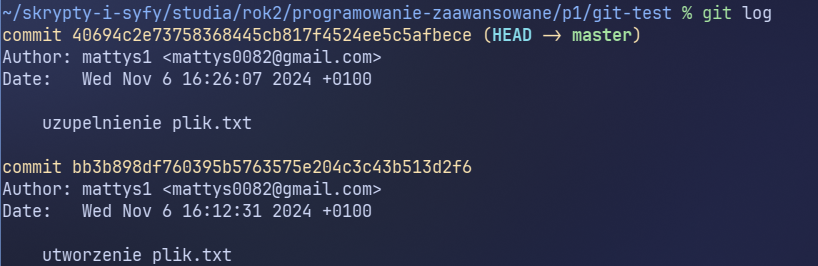
\includegraphics[width=1\textwidth]{images/git_log.png}
	\caption{\centering{Log gita}}
	\label{fig:git_log}
\end{figure}

Jak na rys. \ref{fig:git_log} jest pokazane, używając komendy \texttt{git log}, można wyświetlić log commitów w repozytorium.

\begin{figure}[H]
	\centering
	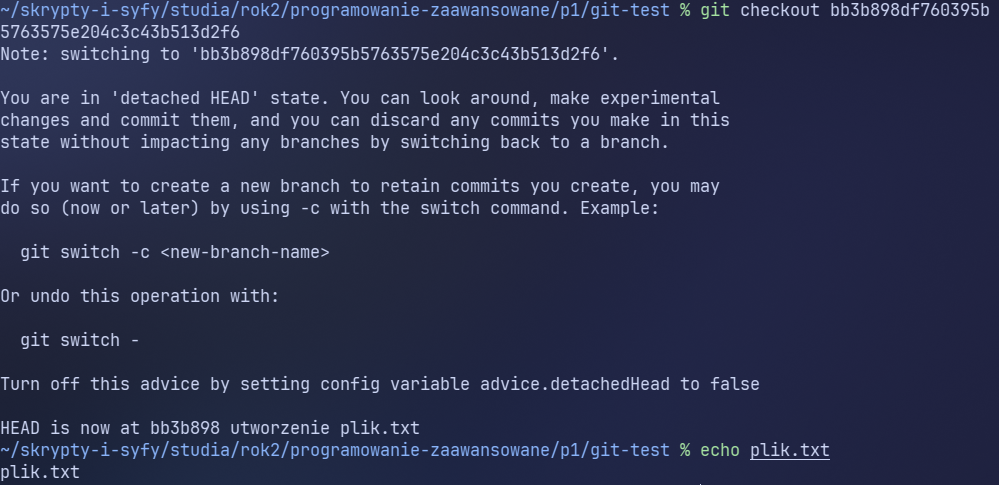
\includegraphics[width=1\textwidth]{images/git_checkout.png}
	\caption{\centering{Demonstracja checkout}}
	\label{fig:git_checkout}
\end{figure}

Jak widać na rys. \ref{fig:git_checkout}, komenda \texttt{git checkout}, pozwala na przejście repozytorium w inny stan, w tym przypadku przechodzi się do commita o danym ID, pokazanym na rys. \ref{fig:git_log}. Jako, że jest to pierwszy commit, nie ma w nim zmian z drugiego.

\subsection{Doxygen}
Doxygen\cite{doxygensite} jest narzędziem automatycznie generującym dokumentację programu z komentarzy w kodzie źródłowym. Potrafi on generować strony HTML, gdzie można dynamicznie nawigować się miedzy rożnymi częściami kodu oraz pliki \LaTeX, które można konwertować na różne, statyczne formaty.

\subsection{Github Copilot}

GitHub Copilot\cite{copilotsite} to model \texttt{LLM} oferowany przez GitHub - może on analizować kod źródłowy i funkcjonować jako zaawansowany autocompleter lub asystent potrafiący tworzyć proste fragmenty. Jest on bezpośrednio zintegrowany z wieloma narzędziami Microsoftu, takimi jak Visual Studio Code czy zwykłe Visual Studio. Jednak, jest on dostępny również jako rozszerzenie do innych edytorów, jak Neovim, którego instalacja przy użyciu menagera pluginów \texttt{Lazygit} jest ukazana na rys. \ref{fig:copilot_install}.

\begin{figure}[H]
	\centering
	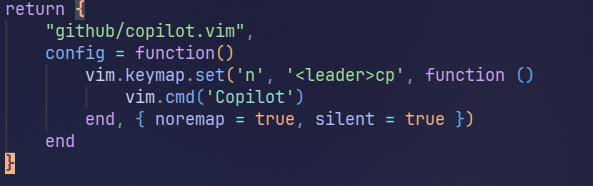
\includegraphics[width=1\textwidth]{images/copilot-plugin.png}
	\caption{\centering{Plik instalacyjny Plugina Copilot}}
	\label{fig:copilot_install}
\end{figure}

W Visual Studio jest on zainstalowany domyślnie.

\subsection{ChatGPT}

ChatGPT\cite{chatgptsite} jest serią modeli LLM oferowanych przez firmę OpenAI. W przeciwieństwie do Copilota jest on modelem bardziej skoncentrowanym na ogólnej tematyce, aniżeli na programowaniu. Jest on głównie nastawiony na funkcje czatu, ale oferowane jest też API do integracji z innymi narzędziami. Wygląd strony głównej zawarty jest na rysunku nr. \ref{fig:chatgptsite}.

\begin{figure}[H]
	\centering
	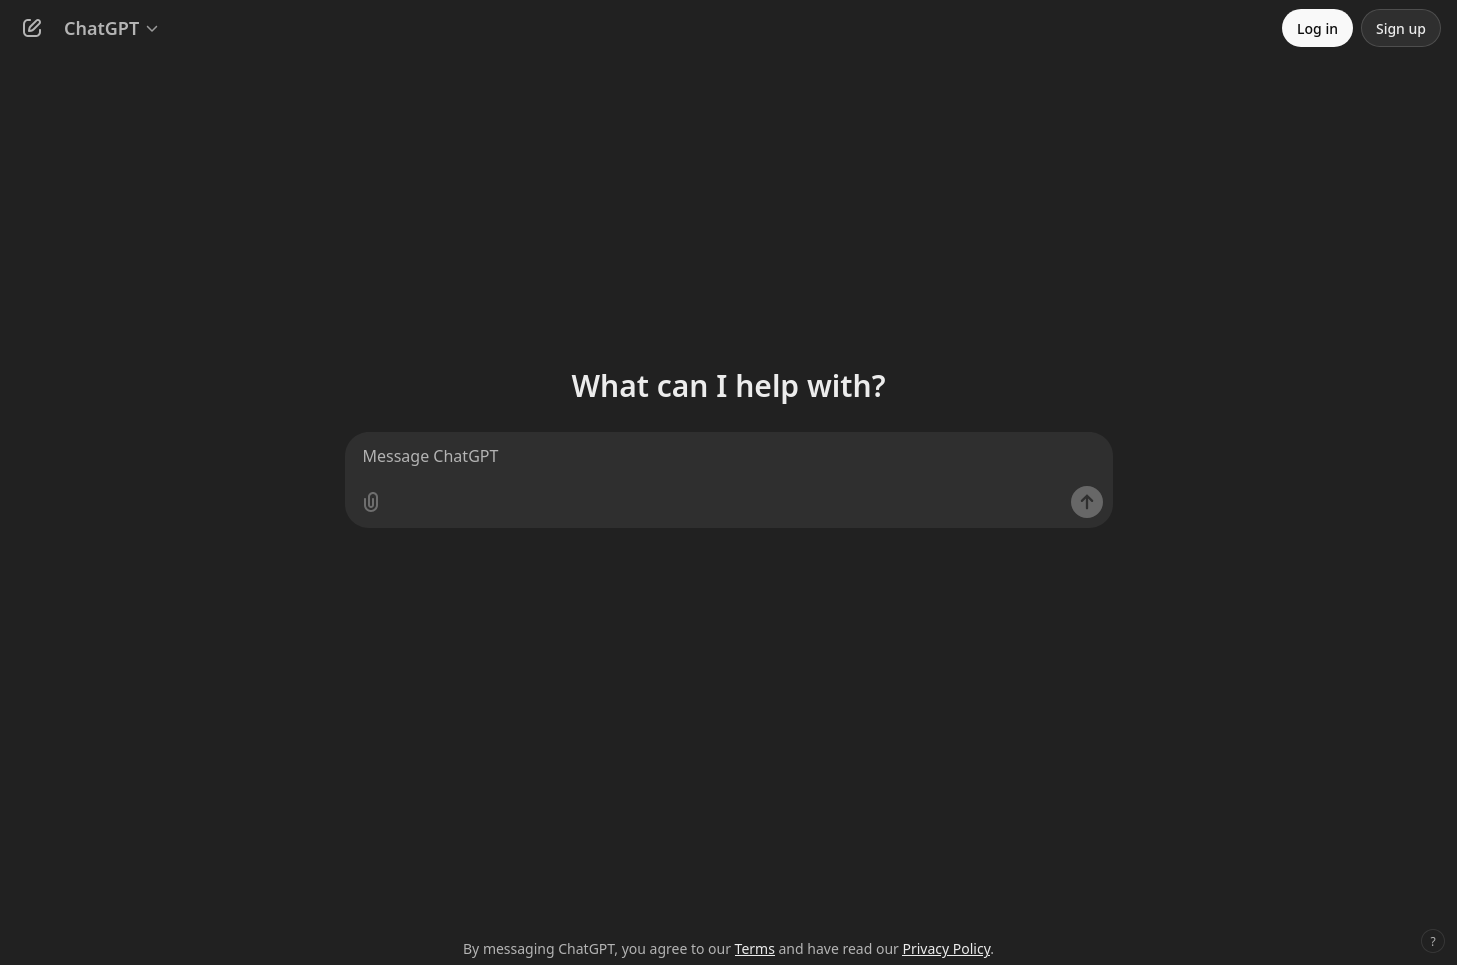
\includegraphics[width=1\textwidth]{images/chatgpt_site.png}
	\caption{\centering{Strona główna ChatGPT}}
	\label{fig:chatgptsite}
\end{figure}
